%% SOURCE: experiments/010-kuzmin-tmi/scripts/pcl6_deletion_paths.py -- path frame from results/pcl6_deletion_paths.csv, triple frame from results/pcl6_deletion_paths_triples.csv, counts from results/pcl6_deletion_paths_summary.json

\section{Walking the screen: every measured deletion path\secstatus{todo}}

The panel design asks for a triple whose deletions do not cost fitness on the way
in. That is a claim about a \emph{route}, not about an endpoint, and it is
testable without building anything, because the whole lattice under the
\texttt{YER059W} screen is already measured.

\subsection{The lattice is complete for this one screen\secstatus{todo}}

Every \texttt{YER059W} record comes from the query double \texttt{YER059W} +
\texttt{YIL050W}, so every triple in it is $\{\emph{PCL6}, \emph{PCL7}, X\}$ for
an array gene $X$. Stacking deletions one at a time makes each triple reachable
by six orderings, and each ordering is a four-rung ladder,
\[
\text{WT } (f = 1) \;\longrightarrow\; \text{single } a \;\longrightarrow\;
\text{double } \{a,b\} \;\longrightarrow\; \text{triple } \{i,j,k\}.
\]
A route has \textbf{no backwards move} when every deletion leaves fitness at
least as high as the strain before it. That is the question a strain build
actually faces: stacking one deletion at a time and keeping only improvements,
which triples can be reached at all.

Of 1{,}097 trigenic records, 919 carry a deletion array and 178 a
temperature-sensitive allele; deletions are the set used here. Requiring all
three singles and all three doubles leaves 917 triples and 5{,}502 paths. Each
rung is a published measurement, sourced per rung: the triple and the paralog
double from \texttt{TmfKuzmin2020} in screen, the mixed doubles from
\texttt{DmfKuzmin2020} with \texttt{DmfCostanzo2016} at 30~C filling the
remainder, the singles from \texttt{SmfKuzmin2020} on the same rule.

The two single-mutant sources disagree on the query genes, and the disagreement
decides a sign. Kuzmin gives \emph{pcl6} 0.9153 and \emph{pcl7} 0.8956; Costanzo
gives 1.0245 and 0.9950. Against the measured double at 0.9063 the digenic term
is $+0.0866$ on the first pair and $-0.1131$ on the second. Kuzmin's singles are
used, because they share a normalization with the double and the triple standing
above them in the same ladder.

\subsection{The ladder does not climb\secstatus{todo}}

\begin{table}[H]
\centering
\footnotesize
\begin{tabular}{lrr}
\toprule
Criterion & Paths of 5{,}502 & Triples of 917 \\
\midrule
No backwards move                        & 3   & 3   \\
No step below 1 SE                       & 228 & 188 \\
No backwards move after the first deletion & 428 & n/a \\
\bottomrule
\end{tabular}
\caption{Accessibility of the 917 complete triples under the
\emph{pcl6}$\Delta$ \emph{pcl7}$\Delta$ query. Generated by
\protect\file{experiments/010-kuzmin-tmi/scripts/pcl6\_deletion\_paths.py}.}
\end{table}

The first deletion alone ends 90.3 percent of paths, because the median array
single sits at 0.973 and both query singles sit near 0.90. Of the survivors the
second deletion removes a further 54 percent. Three paths clear all three steps,
and all three open with the array gene rather than a query gene, since deleting
\emph{PCL6} or \emph{PCL7} costs fitness on its own: \emph{kar9} then
\emph{pcl7} then \emph{pcl6} at 1.0587, \emph{nuc1} then \emph{pcl6} then
\emph{pcl7} at 1.0258, and \emph{chs7} then \emph{pcl7} then \emph{pcl6} at
1.0260. None is a called interaction at $P < 0.05$, the closest being
\emph{kar9} at $P = 0.0502$.

\subsection{A positive interaction is not a fitter strain\secstatus{todo}}

43 of the 917 triples finish above wild type, the best at 1.0834. Twelve carry a
called positive interaction at $\tau > +0.08$ with $P < 0.05$, and exactly one of
those twelve also finishes above wild type: \emph{puf4} (\texttt{YGL014W}),
$\tau = +0.086$ at $P = 0.022$, endpoint 1.0834, with two of its six routes
staying within 1 SE of never stepping back.

The rest of the called set runs the other way. \emph{pho80} (\texttt{YOL001W})
carries the second largest $\tau$ in the screen, $+0.324$ at $P = 0.0004$, and
finishes at 0.2852. Pho80p is the cyclin partner of Pho85p, of which \emph{PCL6}
and \emph{PCL7} are two further cyclins, so the interaction sits where a
mechanism would put it. Positive $\tau$ there means the triple is less sick than
the multiplicative expectation, not that it is healthy. Across all 917 triples
$\tau$ and endpoint fitness correlate at $r = +0.14$.

Selecting on interaction and selecting on fitness are therefore close to
independent in this screen. A panel ranked on predicted $\tau$ alone returns
mostly sick strains, and the fitness constraint has to enter the objective rather
than be applied as a filter afterwards.

\subsection{The strong tier and the fitness goal are disjoint\secstatus{todo}}

Raising the cut does not fix this; it makes it worse, and the crossover is
already below the strong tier. Every triple clearing $\tau > +0.16$ with
$P < 0.05$ finishes below wild type, and none of them has a route that avoids a
backwards move even after allowing 1 SE of slack.

\begin{table}[H]
\centering
\footnotesize
\begin{tabular}{lrrrrr}
\toprule
$\tau$ cut & Criterion & Triples & Best $f_{ijk}$ & Above WT & With a route \\
\midrule
$+0.08$ & called ($P<0.05$) & 12  & 1.0834 & 1  & 4  \\
$+0.08$ & magnitude only    & 152 & 1.0834 & 12 & 48 \\
$+0.12$ & called ($P<0.05$) & 7   & 0.9822 & 0  & 2  \\
$+0.12$ & magnitude only    & 96  & 1.0734 & 7  & 25 \\
$+0.16$ & called ($P<0.05$) & 3   & 0.8662 & 0  & 0  \\
$+0.16$ & magnitude only    & 69  & 1.0734 & 7  & 17 \\
$+0.20$ & called ($P<0.05$) & 3   & 0.8662 & 0  & 0  \\
$+0.20$ & magnitude only    & 58  & 1.0734 & 4  & 11 \\
\bottomrule
\end{tabular}
\caption{What each interaction tier costs in fitness. ``With a route'' counts
triples having at least one of six orderings that never steps back by more than
1 SE. Generated by
\protect\file{experiments/010-kuzmin-tmi/scripts/pcl6\_deletion\_paths.py}.}
\end{table}

The three strong triples are \emph{ubp15} at $\tau = +0.357$ finishing at 0.686,
\emph{pho80} at $+0.324$ finishing at 0.285, and \emph{rad57} at $+0.201$
finishing at 0.866. Dropping the significance requirement recovers fitness but
abandons the call: 69 triples clear $+0.16$ on magnitude alone and 7 of those
beat wild type, none of them at $P < 0.05$.

\begin{figure}[H]
\centering
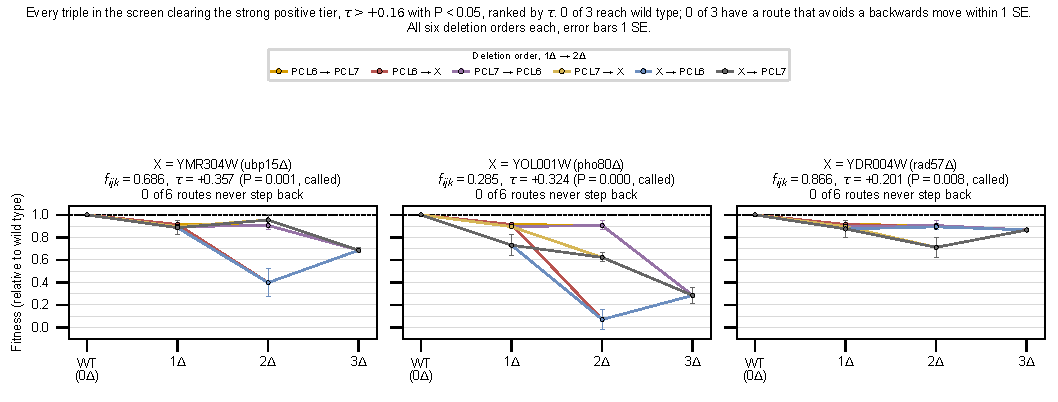
\includegraphics[width=\linewidth]{figures/pcl6_deletion_path_panels_strong.pdf}
\caption{Every triple in the screen clearing the strong positive tier, all six
deletion orders each. Generated by
\protect\file{experiments/010-kuzmin-tmi/scripts/pcl6\_deletion\_paths.py}.}
\end{figure}

\begin{figure}[H]
\centering
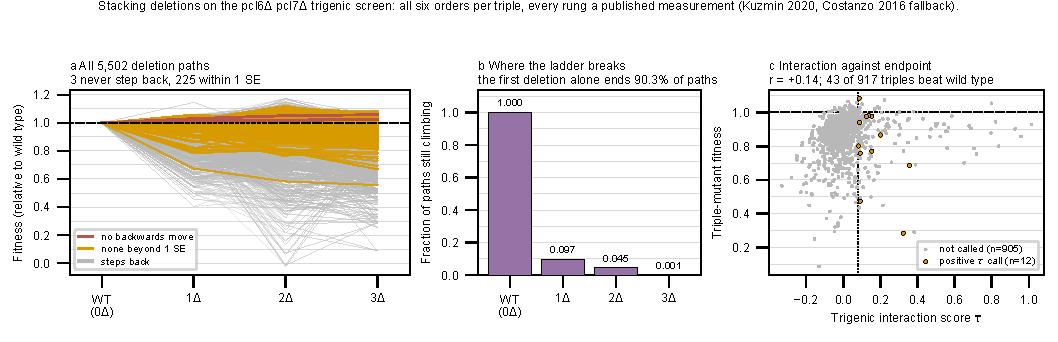
\includegraphics[width=\linewidth]{figures/pcl6_deletion_paths_all.pdf}
\caption{All 5{,}502 measured deletion paths through the \emph{pcl6}$\Delta$
\emph{pcl7}$\Delta$ screen, the step at which each route stops climbing, and
trigenic interaction against endpoint fitness. Generated by
\protect\file{experiments/010-kuzmin-tmi/scripts/pcl6\_deletion\_paths.py}.}
\end{figure}

\begin{figure}[H]
\centering
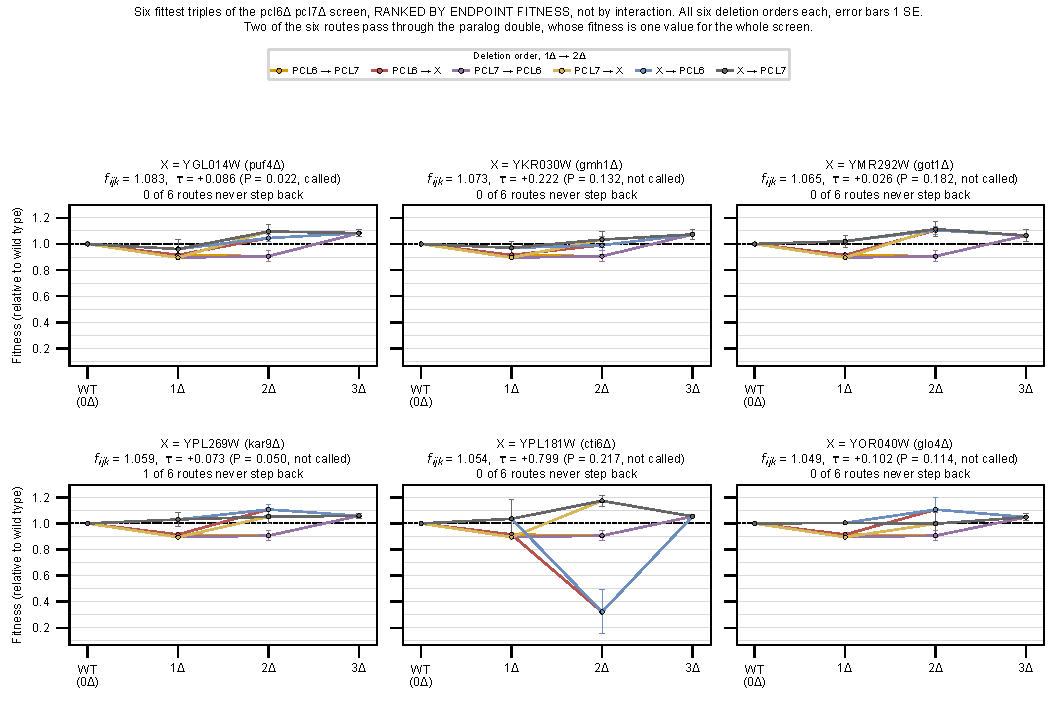
\includegraphics[width=\linewidth]{figures/pcl6_deletion_path_panels.pdf}
\caption{The six highest-fitness triples of the screen, all six deletion orders
each, error bars 1 SE. Two of the six routes pass through the paralog double,
whose fitness is one value for the whole screen. Generated by
\protect\file{experiments/010-kuzmin-tmi/scripts/pcl6\_deletion\_paths.py}.}
\end{figure}
